\documentclass{beamer}
\usepackage{amsmath, graphicx, listings, color, caption}

%% \setlength{\topmargin}{0 mm}
%% \setlength{\oddsidemargin}{5 mm}
%% \setlength{\evensidemargin}{5 mm}
%% \setlength{\textwidth}{150 mm}
%% \setlength{\textheight}{210 mm}

%
\newcommand{\calo}{{\cal O}}
%
\newcommand{\ab}{{\bf a}}
\newcommand{\bb}{{\bf b}}
\newcommand{\db}{{\bf d}}
\newcommand{\eb}{{\bf e}}
\newcommand{\fb}{{\bf f}}
\newcommand{\gb}{{\bf g}}
\newcommand{\ib}{{\bf i}}
\newcommand{\jb}{{\bf j}}
\newcommand{\nb}{{\bf n}}
\newcommand{\pb}{{\bf p}}
\newcommand{\tb}{{\bf t}}
\newcommand{\rb}{{\bf r}}
\newcommand{\xb}{{\bf x}}
\newcommand{\yb}{{\bf y}}
\newcommand{\zb}{{\bf z}}
\newcommand{\qb}{{\bf q}}
\newcommand{\ub}{{\bf u}}
\newcommand{\vb}{{\bf v}}
\newcommand{\wb}{{\bf w}}

\newcommand{\Ab}{{\bf A}}
\newcommand{\Bb}{{\bf B}}
\newcommand{\Eb}{{\bf E}}
\newcommand{\Fb}{{\bf F}}
\newcommand{\Ib}{{\bf I}}
\newcommand{\Hb}{{\bf H}}
\newcommand{\Kb}{{\bf K}}
\newcommand{\Lb}{{\bf L}}
\newcommand{\Pb}{{\bf P}}
\newcommand{\Qb}{{\bf Q}}
\newcommand{\Rb}{{\bf R}}
\newcommand{\Ub}{{\bf U}}
\newcommand{\Tb}{{\bf T}}
\newcommand{\Xb}{{\bf X}}

\newcommand{\uh}{\hat{u}}
\newcommand{\vh}{\hat{v}}
\newcommand{\ph}{\hat{p}}
\newcommand{\qh}{\hat{q}}

\newcommand{\psib}{{\bf \psi}}

\newcommand{\re}{{\rm Re}\,}
\newcommand{\im}{{\rm Im}\,}

\renewcommand{\arraystretch}{1.3}
%
\newcommand{\p}{\partial}
%
\newcommand{\eq}{\!\!\! = \!\!\!}
\newcommand{\om}{\omega}
\newcommand{\divergence}{\nabla\cdot}
\newcommand{\curl}{\nabla\times}

\newcommand{\rhob}{\boldsymbol{\rho}}
\newcommand{\kab}{\boldsymbol{\kappa}}
\newcommand{\etab}{\boldsymbol{\eta}}
\newcommand{\zetab}{\boldsymbol{\zeta}}
\newcommand{\sigmab}{\boldsymbol{\sigma}}
\newcommand{\omegab}{\boldsymbol{\omega}}
\newcommand{\Gb}{{\bf G}}
\newcommand{\kb}{{\bf k}}
\newcommand{\sbold}{{\bf s}}

\title{A small quantum control problem}
\author{N. Anders Petersson}
\institute{Lawrence Livermore National Laboratory\footnote{LLNL-PRES-abcdef;
This work was performed under the auspices of the U.S. Department of
Energy by Lawrence Livermore National Laboratory under Contract DE-AC52-07NA27344. Lawrence Livermore National Security, LLC.}}
\date{\today}

\begin{document}
\lstset{language=[03]Fortran}
% to show file name, caption on bottom, framed.
% How to change the caption label further?
\lstset{
  caption=\lstname, captionpos=t, frame=single, basicstyle=\ttfamily\scriptsize,
  columns=fullflexible, keywordstyle=\color{blue},
  commentstyle=\color{red}, stringstyle=\color{gray},
  showspaces=false,
  showstringspaces=false, breaklines=true
}
\renewcommand\lstlistingname{File}
\renewcommand{\thelstlisting}{}
%%%%%%%%%%%%%%%
\frame{\titlepage}

%%%%%%%%%%%%%%%
\begin{frame}{A 2-qubit gate}
  We want to design a gate that transforms
  \[
  |\ub\rangle = a|00\rangle + b|01\rangle + c|10\rangle + d|11\rangle
  \]
  into
  \[
  |\vb\rangle = b|00\rangle + a|01\rangle + c|10\rangle + d|11\rangle
  \]
  This operation can be described in matrix notation as
  \[
  \vb = P \ub,\quad
  P = \begin{pmatrix}
    0 & 1 & 0 & 0\\
    1 & 0 & 0 & 0\\
    0 & 0 & 1 & 0\\
    0 & 0 & 0 & 1
    \end{pmatrix}
  \]
  Note that $P$ is unitary.
\end{frame}


%%%%%%%%%%%%%%%%%%%%%%
\begin{frame}{An example}
  \begin{figure}
    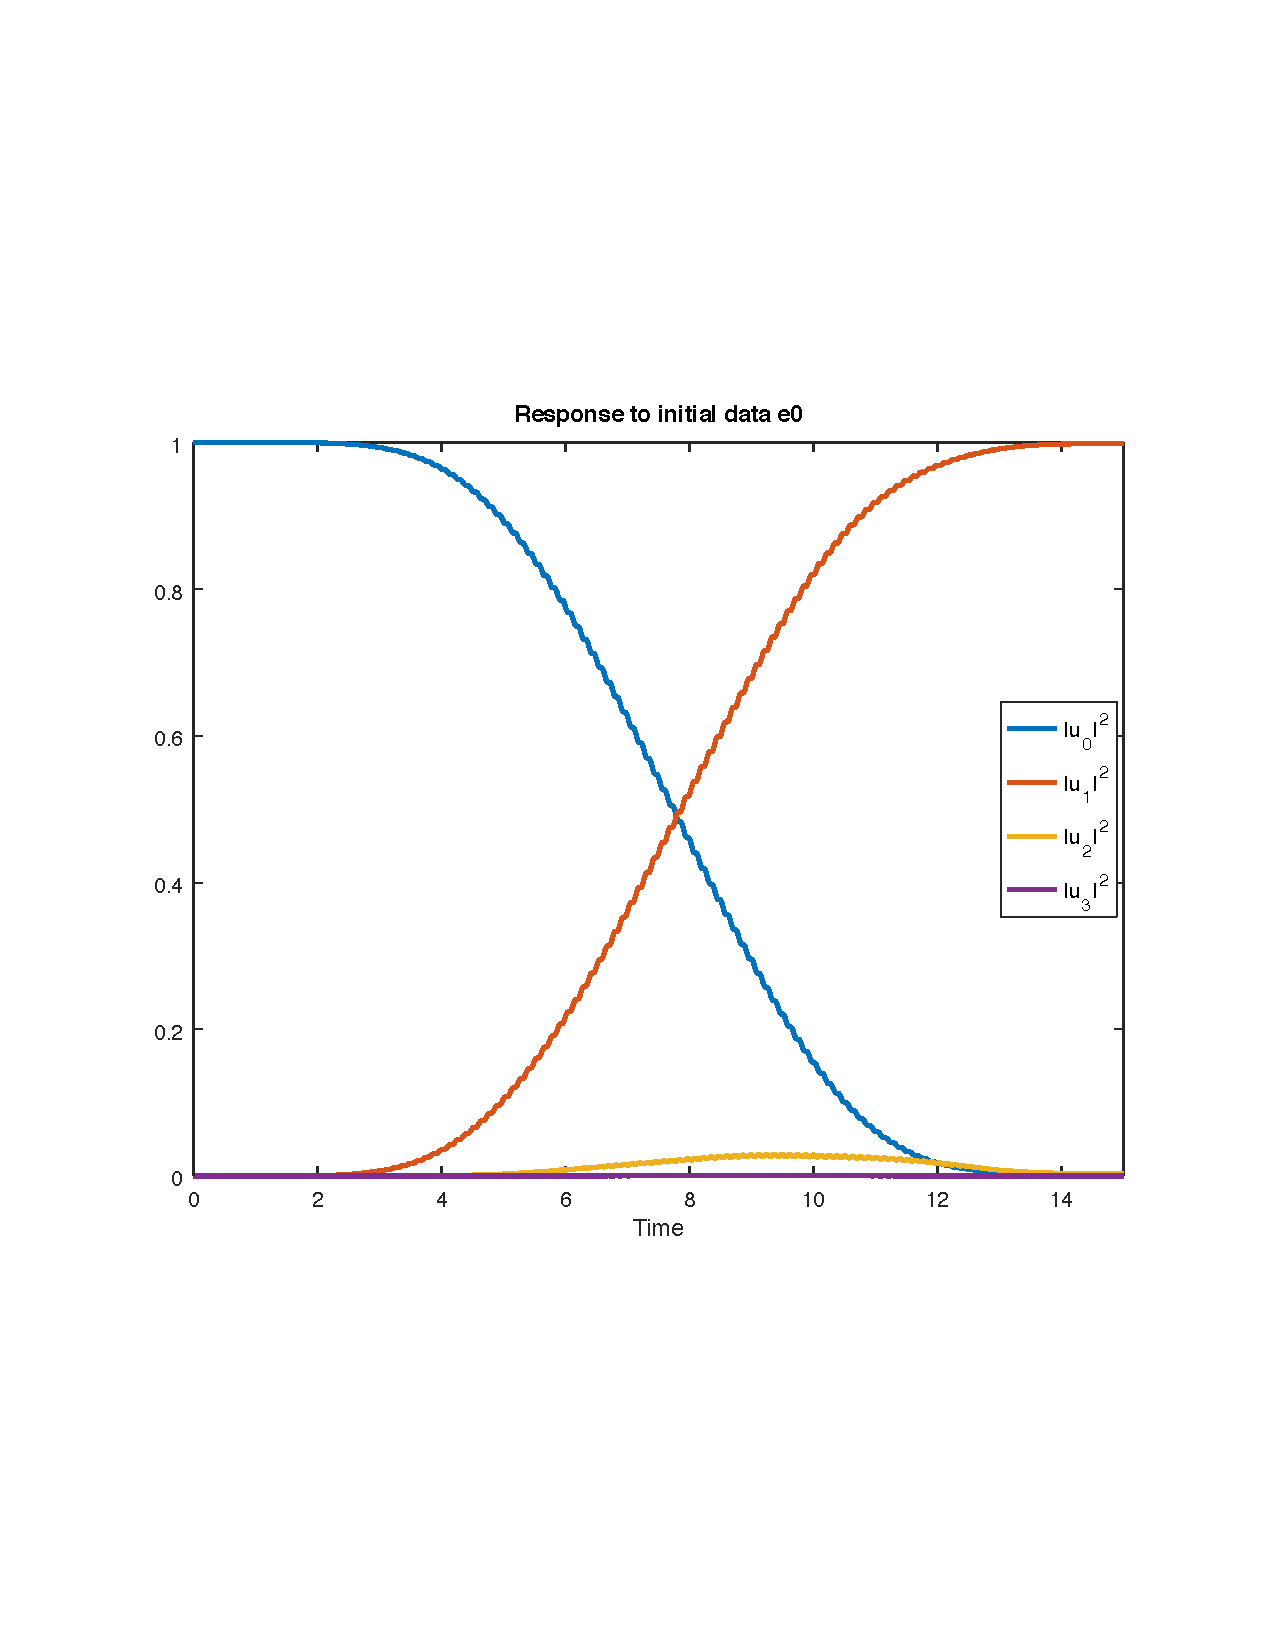
\includegraphics[width=0.45\linewidth]{resp0.pdf}\hspace{3mm}
    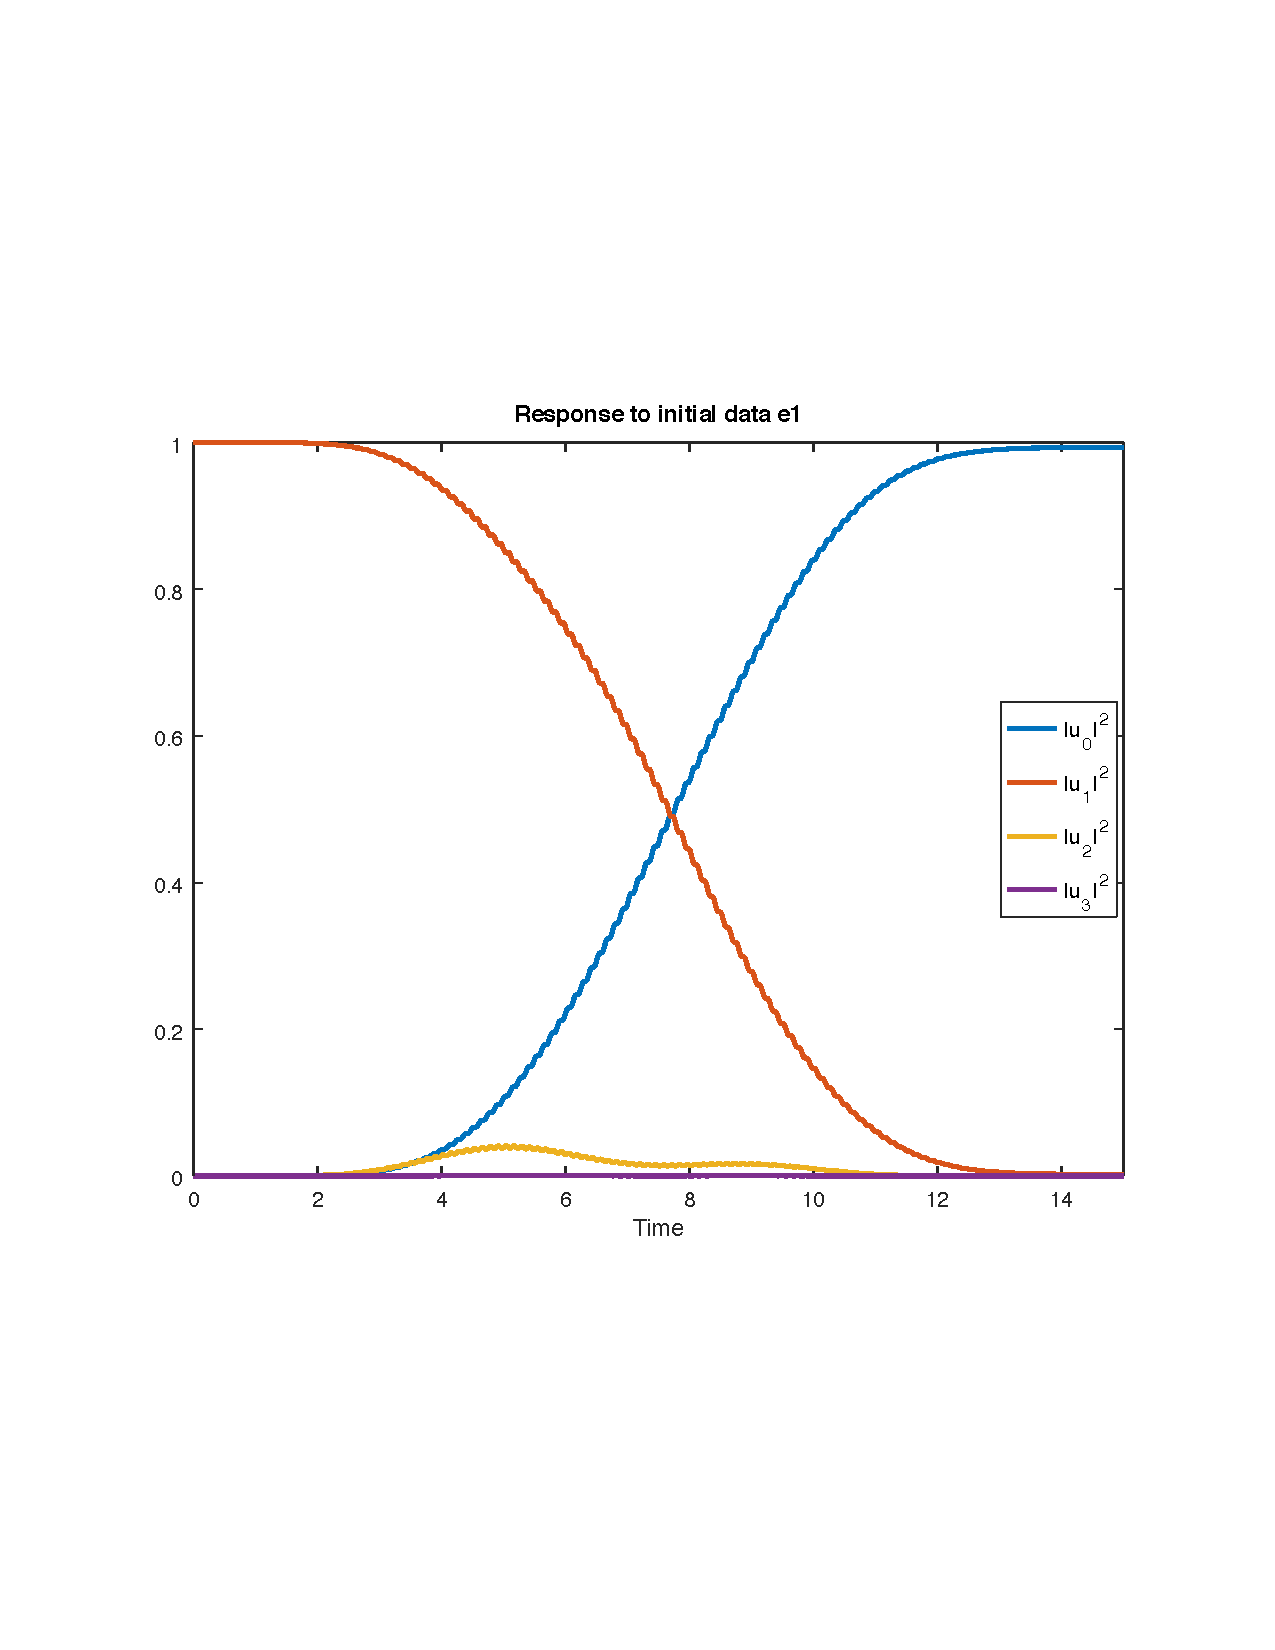
\includegraphics[width=0.45\linewidth]{resp1.pdf}\\
    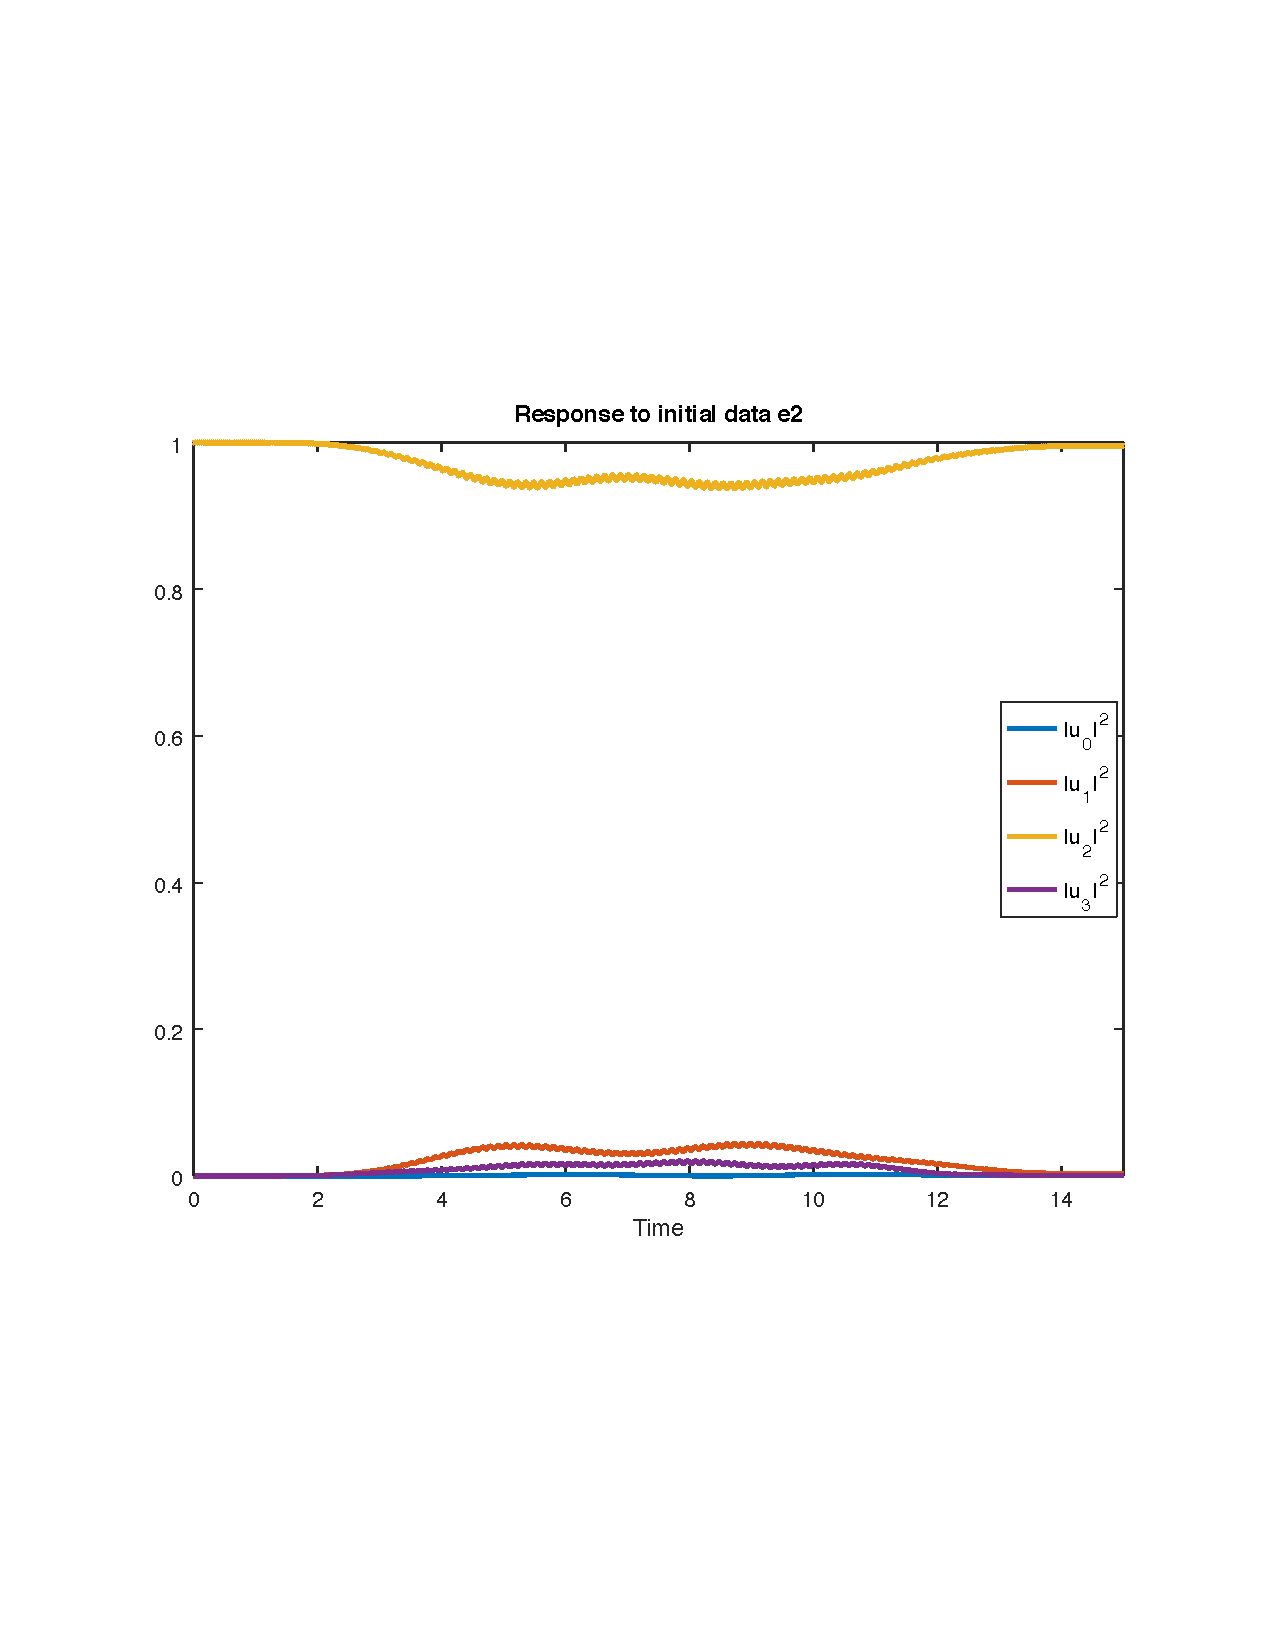
\includegraphics[width=0.45\linewidth]{resp2.pdf}\hspace{3mm}
    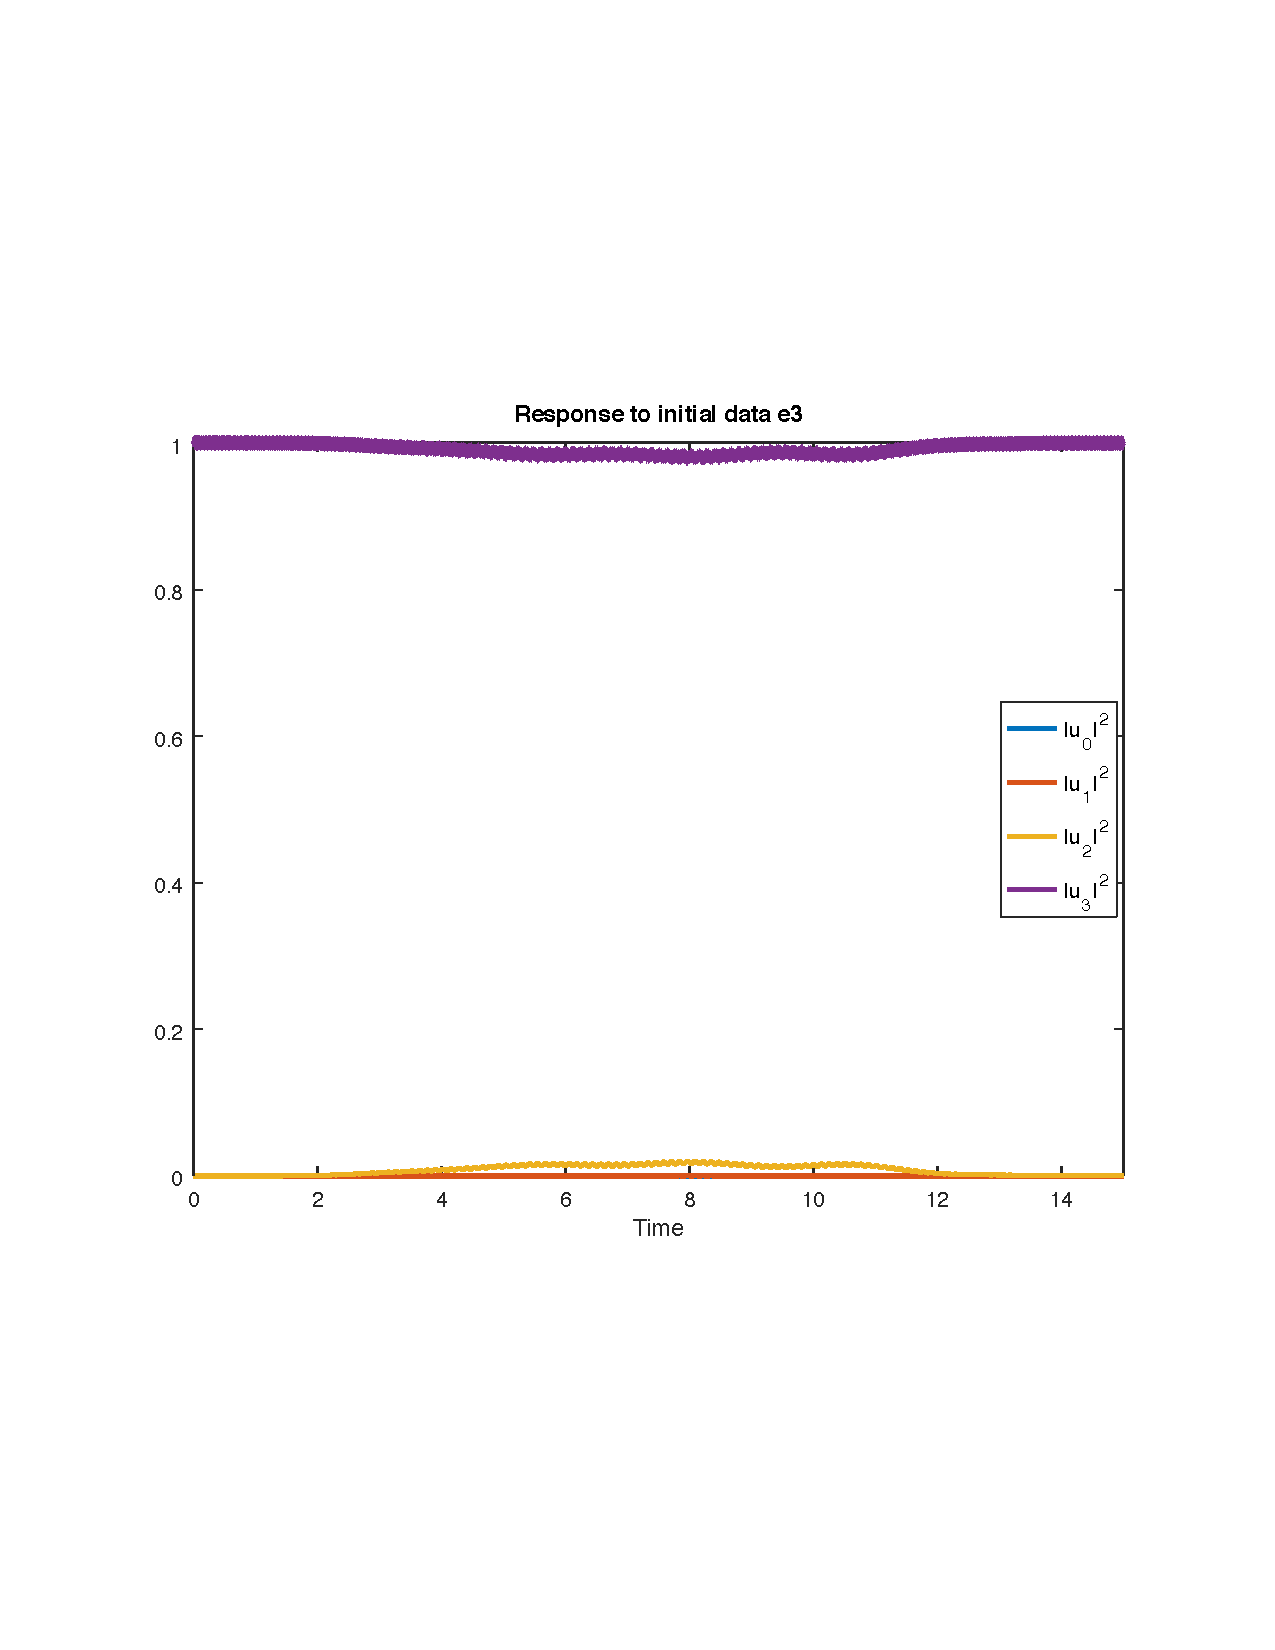
\includegraphics[width=0.45\linewidth]{resp3.pdf}
  \end{figure}
\end{frame}

%%%%%%%%%%%%%%%%%%%%%%
\begin{frame}{The control problem}
 The quantum state is governed by the ODE
  \[
  \dot{\Psi}_k = i(H_0 + p(t)H_c)\Psi_k,\quad
  t\in[0,T], \quad \Psi_k(0) = \eb_k,
  \]
  for $k=1,2,3,4$, where $\Psi_k \in {\mathbb C}^4$ and 
  \[
  H_0=\mbox{diag$(0, \omega_1, \omega_2, \omega_3)$},\quad
  H_c=\begin{pmatrix}
  0 & 1 & 0 & 0 \\
  1 & 0 & \sqrt{2} & 0\\
  0 & \sqrt{2} & 0 & \sqrt{3} \\
  0 & 0 & \sqrt{3}& 0
  \end{pmatrix}
  \]
  The formal (unitary) solution operator is
  \[
  \Psi_k(T) = U \eb_k,\quad
%
  U = e^{iH_0T} e^{i\int_0^T p(\tau)\,d\tau\, H_c}
  \]
  Challenge: Determine the control function $p(t)$ such that $U=P$.
\end{frame}

%%%%%%%%%%%%%%%%%%%%%%
\begin{frame}{Optimization problem}
  Expand the control function in a basis $p_k$,
  \[
  p(t) = \sum_{k=1}^M \alpha_k p_k(t)
  \]
  Let $\db_k=P\eb_k$ be the target state.

  Minimize the functional
  \[
  g(\Psi) = \sum_{k=1}^4 \int_0^T w_k(\tau) \left( |\Psi_k(\tau)|^2 -
  |\db_k|^2\right)^2\, d\tau,\quad w_k(T) = 1,
  \]
  under the constraint that $\Psi_k$ satisfies the above ODE.
\end{frame}

%%%%%%%%%%%%%%%%%%%%%%
\begin{frame}{Designing the control function}
  The basis functions (induce resonance),
  \begin{align*}
    p_{2q-1}(t) = \cos(\omega_1 t) f_q(t),\\
    p_{2q}(t) = \sin(\omega_1 t) f_q(t).
  \end{align*}
  The first 4 functions $f_q(t)$:
  \begin{figure}
    \includegraphics[width=0.5\linewidth]{btf.pdf}
  \end{figure}
\end{frame}

%%%%%%%%%%%%%%%%%%%%%%
\begin{frame}{Numerical solution approach}
  \begin{itemize}
    \item Discretize the ODE by Leap-Frog (2nd order accurate, energy
      stable)
    \item Evaluate cost function $g(\Psi)$ by solving the ODE for 4 initial conditions
    \item Evaluate gradient $\nabla_\alpha g$ by solving the ODE
      forwards, backwards, together with the adjoint ODE
    \item Start with 1 parameter and do a line search for optima: $\alpha_{10}$
    \item For 2 parameters, start from $(\alpha_{10},0)$ and call {\bf
      sqp} (sequential quadratic programming) in octave. New optima: $(\alpha{11},\alpha{21}$.
    \item Add polynomials on next level, do an 8 parameter
      optimization starting from previous $\alpha$.
    \item Keep adding polynomials until cost function is sufficiently small.      
  \end{itemize}
\end{frame}
\end{document}

